\seccion{Probabilidades}
\label{Sec:MP:Probabilidad}

El  concepto  de  {\it  probabilidad}  es importante  en  situaciones  donde  el
resultado de un  dado proceso o medici\'on es incierto, cuando  la salida de una
experiencia no  es totalmente  previsible. La probabilidad  de un evento  es una
medida que se asocia con cu\'an probable es el evento o resultado.

Una  definici\'on  de probabilidad  se  puede dar  en  base  a la  enumeraci\'on
exhaustiva de los resultados posibles de un experimento o proceso,
%lo que no siempre es factible
suponiendo que el conjunto de posibilidades es completo en el sentido de que una
de ellas  debe ocurrir  o debe ser  verdad. Si  el proceso tiene  $K$ resultados
distinguibles,  mutuamente excluyentes e  igualmente probables  (esto es,  no se
prefiere una posibilidad frente a otras), y si $k$ de esos $K$ resultados tienen
un dado atributo,  la probabilidad asociada a dicho atributo  en un dado proceso
es $\frac{k}{K}$. Por  ejemplo, sorteando un n\'umero entre  los naturales del 1
al 10, la probabilidad de ``obtener un n\'umero par'' es $\frac5{10} = \frac12$.

Otra  definici\'on  de  probabilidad  se  basa  en  la  frecuencia  relativa  de
ocurrencia  de  un evento.   Si  en  una cantidad  $K$  muy  grande de  procesos
independientes  cierto   atributo  aparece  $k$   veces,  se  identifica   a  la
probabilidad  asociada a  un  proceso o  ensayo  con la  frecuencia relativa  de
ocurrencia    $\frac{k}{K}$    del    atributo~\cite[\&   Ref.]{Bra76,    Hal90,
  ShaVov06}.
%~\footnote{A  pesar de  que las  nociones de  azar (que  proviene del
%  \'arabe {\it  zahr} que significa dado,  flor) o de  aleatoriedad (del lat\'in
%  {\it alea} que es suerte, dado) son muy antiguas~\cite{Ser00}, el matem\'atico
%  italiano y jugador de dados y cartas Gerolamo Cardano es ``probablemente'' uno
%  de los primeros en tratar  matem\'aticamente el concepto de probabilidad en el
%  siglo~{XVI},  en su  libro  sobre los  juegos  de azar  escrito  en 1564  pero
%  publicado  en   1663~\cite{Car63}  (ver~\cite{Bel05}  o~\cite[Cap.~4]{Hal90}).
%  Entre  los  numerosos  matem\'aticos  que  desarrollaron la  teor\'ia  de  las
%  probabilidades,  en  particular  los  franceses  Pierre  de  Fermat  y  Blaise
%  Pascal~\cite[Cap.~5]{Hal90},  hay  que  mencionar  tambi\'en  al  suizo  Jacob
%  Bernoulli    (miembro   de    una   dinast\'ia    de   matem\'aticos)~\cite[en
%  lat\'in]{Ber1713}   o~\cite{Ber1713:2}  y   al   franco-ingl\'es  Abraham   de
%  Moivre~\cite{Dem56}.   El  franc\'es  Pierre  Simon  Laplace~\cite{Lap20}  fue
%  quiz\'as uno de los primeros en  proveer un aporte importante al desarrollo de
%  la  teor\'ia de las  probabilidades en  los siglos  XVIII-XIX, a  trav\'es del
%  punto de vista ``frecuentista'' y combinatorial (ver tambi\'en~\cite[Caps.~13,
%  15 \&~22]{Hal90}).}.
%lim N->infty n/N indef.

Los axiomas de Kolmogorov
%~\footnote{Un paso importante es debido a Kolmogorov en
%  1933  que  se apoy\'o  sobre  trabajos  de  Richard von  Mises~\cite{Mis32}  y
%  tambi\'en sobre  la teor\'ia de  la medida y  de la integraci\'on,  debidas entre
%  otros a \'Emile Borel y Henri
%%Henri-Leon
%  Lebesgue~\cite{Bor98,   Bor09,   Leb04,   Leb18,   Hal50},   para   formalizar
%  anal\'iticamente  la  teoria   de  las  probabilidades~\cite{Kol56,  BarNov78,
%    JacPro03}.}
proveen requisitos suficientes para  determinar completamente las propiedades de
la medida de probabilidad  $P(A)$ que se puede asociar a un  evento $A$ entre un
conjunto de resultados o eventos de un proceso.

Llamemos $\Omega$ al {\it espacio  muestral} o {\it espacio fundamental}, que es
el  espacio  de {\it  muestras}  ({\it outcomes},  en  ingl\'es)  \ $\omega  \in
\Omega$.  Se asocia  \ $\A$ \ a una colecci\'on de  sub-conjuntos de \ $\Omega$,
donde los  elementos de $\A$ son  llamados {\it eventos}.  Por  ejemplo, para un
dado de 6  caras, $\Omega$ es el  conjunto de caras que se  pueden etiquetar con
los n\'umeros naturales del 1 al 6 (o tambi�n con las letras {\it a, b, c, d, e,
  f}, u otro etiquetado), y $\A$  tiene los eventos $A$ ``es un n\'umero natural
par'' y $B$ ``es un n\'umero natural  impar''.  En el caso de analizar el tiempo
de  vida de  un aparato,  $\Omega \equiv  \Rset_+$.  El  conjunto  de resultados
posibles se supone conocido, a\'un cuando se desconozca de antemano el resultado
de una prueba.

Entre los eventos  se pueden considerar operaciones y  definiciones an\'alogas a
las de la  teor\'ia de conjuntos (ver entre  otros~\cite{Spi76, Bre88, ManWol95,
  Sie75, Sie76, Bor98, Bor09}):
%
\begin{itemize}
\item Combinaci\'on o  uni\'on de eventos: \  $A \cup B$ implica que  se da $A$,
  \'o $B$, o ambos (por ejemplo, para un dado de 6 caras, si $A$ son los eventos
  ``cara par'' y $B$ los eventos ``cara menor o igual a 3'', resulta $A \cup B =
  \{1 \; 2 \; 3 \; 4 \;  6\}$). Seg\'un la literatura, se denota a veces \ $A+B$
  \ o \ $A \vee B$.
%
\item  Intersecci\'on de  eventos:  \ $A\cap  B$  implica que  se dan  ambos
  $A$~y~$B$ (en  el ejemplo precedente,  $A \cap  B = \{  2 \}$). Se  denota a
  veces \ $(A,B)$ \ o \ $A \wedge B$.
%
\item Complemento de un evento: \ $\bar{A}$ indica que no se da $A$. Se denota a
  veces \ $-A$ \ o \ $A^\complement$  (en el ejemplo precedente, $\bar{A} = \{ 1
  \; 3 \; 5 \}$).
%
\item   Eventos  {\it  disjuntos}   o  {\it   mutuamente  excluyentes}   o  {\it
    incompatibles}: \ son aquellos que no se  superponen, se anota \ $A \cap B =
  \emptyset$ \ donde \ $\emptyset =  \bar{\Omega}$ \ denota el {\it evento nulo}
  (evento que no puede ocurrir, es  el complemento de $\Omega$). Por ejemplo los
  eventos ``cara par'' y ``cara impar'' son incompatibles.
%
\item Denotaremos  tambi\'en $A \setminus B$  \ cuando el evento  $A$ se realiza
  pero no  $B$. Se lo  denota tambi\'en \  $A-B$, \ que  es tambi\'en \  $A \cap
  \bar{B}$ (en el ejemplo precedente, $A \setminus B=\{4\}$).
\end{itemize}
%
\noindent Esto  es ilustrado en la Fig.~\ref{Fig:MP:Ensembles}  empleando lo que
se  conoce   como  diagramas  de  Venn~\footnote{Este  tipo   de  diagramas  fue
  popularizado por el ingl�s John  Venn en 1880, pero en su trabajo~\cite{Ven80}
  da la paternidad al matem\'atico suizo  Leonhard Euler, uno de los primeros en
  usar tal  representaci\'on en  el siglo  XVIII en sus  famosas ``Cartas  a una
  princesa alemana,  acerca de diversas  cuestiones de f\'isica  y filosof\'ia''
  (ver~\cite[L~102-105, pp.~95-126]{Eul68}),  o antes a Christian  Weise y Johan
  Christian  Langius~\cite{Lan12};  apareci\'o a\'un  en  trabajos de  Gottfried
  Wilhelm Leibniz en el  siglo anterior.\label{Foot:MP:Euler}}.  La uni\'on y la
intersecci\'on de  eventos satisfacen  las mismas reglas  que en la  teor\'ia de
conjuntos, es decir cada una es conmutativa \ $A \cup B = B \cup A$, \ $A \cap B
= B \cap A$, \ asociativa \ $(A \cup B)  \cup C = A \cup (B \cup C)$, \ $(A \cap
B) \cap C = A \cap (B \cap C)$, \ distributiva con respecto a la otra \ $(A \cup
B) \cap C = (A \cap C) \cup (B \cap  C)$, \ $(A \cap B) \cup C = (A \cup C) \cap
(B  \cup  C)$  \  (ver  por ejemplo~\cite{Jef48,  Jef73,  Hal50,  Fel71,  Bre88,
  ManWol95, IbaPar97, LehCas98, AthLah06, Coh13, HogMck13}).

\begin{figure}[h!]
\begin{center} 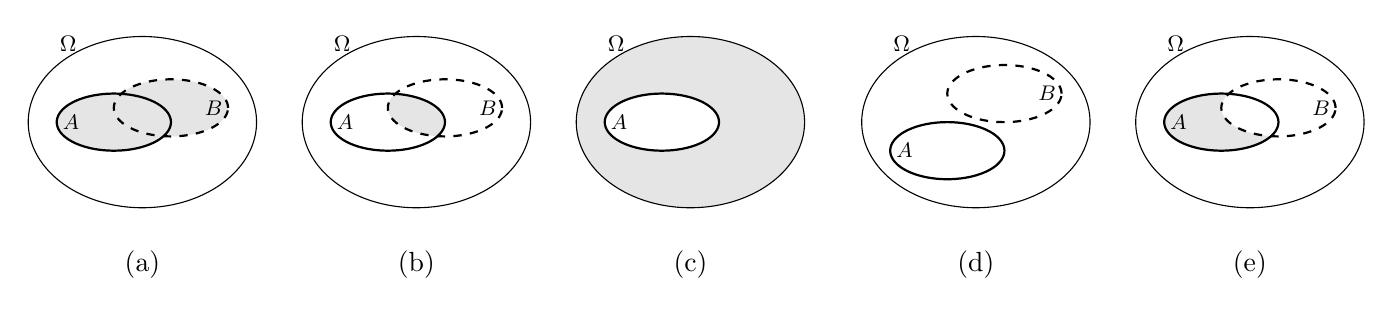
\begin{tikzpicture}[scale=.725]
\shorthandoff{>}
%
% Union y interseccion:
%
% Omega: .25*(x-.25)^2 + (y/1.5)^2 = 1
% A: x^2 + 4 y^2 = 1
% B: (x-1)^2 + 4 (y-1/4)^2 = 1
% A y B se cruzan cuando x = 1 \pm sqrt(55)/10 =>
% theta = acos(.5 \pm sqrt(55)/20) para A
% theta = acos(-.5 \pm sqrt(55)/20) para A
\pgfmathsetmacro{\s}{acos(.5-sqrt(55)/20)};
\pgfmathsetmacro{\t}{-acos(.5+sqrt(55)/20)};
\pgfmathsetmacro{\u}{-acos(-.5+sqrt(55)/20)};
\pgfmathsetmacro{\v}{acos(-.5-sqrt(55)/20)-360};
%
%
%Union
\begin{scope}
%
\fill[opacity=.1]
plot[domain=\s:\t+360,samples=200] ({cos(\x)},{.5*sin(\x)})
-- plot[domain=\u:\v+360,samples=200] ({cos(\x)+1},{.5*sin(\x)+.25})
-- cycle;
%
% borders A, B y Omega
\draw[domain=0:360,samples=200,thick] plot ({cos(\x)},{.5*sin(\x)});
\draw[dashed,domain=0:360,samples=200,thick] plot ({cos(\x)+1},{.5*sin(\x)+.25});
\draw[domain=0:360,samples=200] plot ({2*cos(\x)+.5},{1.5*sin(\x)});
%
% A, B, Omega
\draw (-.75,0) node[scale=.85]{\small $A$};
\draw(1.75,.25) node[scale=.85]{\small $B$};
\draw(-.5,1.375) node[left,scale=.9]{\small $\Omega$};
%
\draw (.5,-2.5) node{(a)};
\end{scope}
%
%
% Interseccion
\begin{scope}[xshift=4.8cm]
%
\fill[opacity=.1]
plot[domain=\s:\t,samples=200] ({cos(\x)},{.5*sin(\x)})
-- plot[domain=\u:\v,samples=200] ({cos(\x)+1},{.5*sin(\x)+.25})
-- cycle;
%
% borders A, B y Omega
\draw[domain=0:360,samples=200,thick] plot ({cos(\x)},{.5*sin(\x)});
\draw[dashed,domain=0:360,samples=200,thick] plot ({cos(\x)+1},{.5*sin(\x)+.25});
\draw[domain=0:360,samples=200] plot ({2*cos(\x)+.5},{1.5*sin(\x)});
%
% A, B, Omega
\draw (-.75,0) node[scale=.85]{\small $A$};
\draw(1.75,.25) node[scale=.85]{\small $B$};
\draw(-.5,1.375) node[left,scale=.9]{\small $\Omega$};
%
\draw (.5,-2.5) node{(b)};
\end{scope}
%
%
% Complemento
\begin{scope}[xshift=9.6cm]
%
\fill[opacity=.1]
plot[domain=0:360,samples=200] ({2*cos(\x)+.5},{1.5*sin(\x)})
-- plot[domain=0:360,samples=200] ({cos(\x)},{-.5*sin(\x)})
-- cycle;
%
% borders A y Omega
\draw[domain=0:360,samples=200,thick] plot ({cos(\x)},{.5*sin(\x)});
\draw[domain=0:360,samples=200] plot ({2*cos(\x)+.5},{1.5*sin(\x)});
%
% A, Omega
\draw (-.75,0) node[scale=.85]{\small $A$};
\draw(-.5,1.375) node[left,scale=.9]{\small $\Omega$};
%
\draw (.5,-2.5) node{(c)};
\end{scope}
%
%
% Excluyentes
\begin{scope}[xshift=14.6cm]
%
% borders A, B (con un shift...) y Omega
\draw[domain=0:360,samples=200,thick] plot ({cos(\x)},{.5*sin(\x)-.5});
\draw[dashed,domain=0:360,samples=200,thick] plot ({cos(\x)+1},{.5*sin(\x)+.5});
\draw[domain=0:360,samples=200] plot ({2*cos(\x)+.5},{1.5*sin(\x)});
%
% A, B, Omega
\draw (-.75,-.5) node[scale=.85]{\small $A$};
\draw (1.75,.5) node[scale=.85]{\small $B$};
\draw(-.5,1.375) node[left,scale=.9]{\small $\Omega$};
%
\draw (.5,-2.5) node{(d)};
\end{scope}
%
%
% privado
\begin{scope}[xshift=19.4cm]
%
\fill[opacity=.1]
plot[domain=\s:\t+360,samples=200] ({cos(\x)},{.5*sin(\x)})
-- plot[domain=\u:\v,samples=200] ({cos(\x)+1},{.5*sin(\x)+.25})
-- cycle;
%
% borders A, B y Omega
\draw[domain=0:360,samples=200,thick] plot ({cos(\x)},{.5*sin(\x)});
\draw[dashed,domain=0:360,samples=200,thick] plot ({cos(\x)+1},{.5*sin(\x)+.25});
\draw[domain=0:360,samples=200] plot ({2*cos(\x)+.5},{1.5*sin(\x)});
%
% A, B, Omega
\draw (-.75,0) node[scale=.85]{\small $A$};
\draw(1.75,.25) node[scale=.85]{\small $B$};
\draw(-.5,1.375) node[left,scale=.9]{\small $\Omega$};
%
\draw (.5,-2.5) node{(e)};
\end{scope}
%
\end{tikzpicture} \end{center}
%
\leyenda{Ilustraci\'on de las operaciones entre eventos: (a)~uni\'on $A \cup B$,
  (b)~intersecci\'on   $A  \cap   B$,  (c)~complemento   $\bar{A}$,  (d)~eventos
  excluyentes  $A  \cap  B  =  \emptyset$,  \ y  (e)~$A  \setminus  B$.  $A$  es
  representado en l\'inea  llena, $B$ en l\'inea discontinua;  en (a)-(c) y (e),
  el resultado de la operaci\'on es la zona sombreada.}
\label{Fig:MP:Ensembles}
\end{figure}

Formalmente, se define  de manera abstracta un espacio  medible $(\Omega,\A)$ de
la  manera siguiente  (~\cite{Hal50,  Fel68, Fel71,  Bre88, IbaPar97,  AthLah06,
  Bog07:v1, Coh13}; ver  tambi\'en~\cite[\& Ref.]{BarNov78, Bor98, Sie18, Sie75,
  Sie76} para notas hist\'oricas):
%
\begin{definicion}[Espacio medible]
\label{Def:MP:EspacioMedible}
%
  $(\Omega,  \A)$,  \  formado por  un  espacio  muestral  \  $\Omega$ \  y  una
  colecci\'on \  $\A$ \ de  conjuntos de \  $\Omega$, \ es llamado  {\it espacio
    medible} si satisface los requisitos
  %
  \begin{enumerate}
  \item $\emptyset \in \A$,
  %
  \item si $A \in \A$, entonces \ $\bar{A} \in \A$,
  %
  \item la uni\'on numerable de conjuntos de $\A$ queda en $\A$ ($\A$ es cerrado
    por la uni\'on numerable).
  %
  \end{enumerate}
  %
  Con  estas propiedades,  $\A$  es llamada  una  {\it $\sigma$-\'algebra}.  Los
  elementos de $\A$ son dichos {\it medibles}.
\end{definicion}
%
\noindent Es sencillo mostrar que $\Omega$  tambi\'en est\'a en $\A$, y que $\A$
es cerrado  por la intersecci\'on  numerable.  Un ejemplo  de $\sigma$-\'algebra
sobre \ $\Omega = \{ 1  \; 2 \; 3 \; 4 \; 5 \; 6 \}$  \ puede ser \ $\A = \big\{
\emptyset \; \Omega \; \{ 1 \; 2 \; 3 \} \; \{ 4 \; 5 \; 6 \} \big\}$.

A partir de \ $(\Omega,\A)$, \ se  asocia una noci\'on de probabilidad \ $P$ \ a
un dado  evento. Esta queda  determinada por los siguientes  requisitos llamados
{\it  Axiomas  de Kolmogorov}  (ver  por  ejemplo~\cite{Spi76, Kol56,  ShaVov06,
  Pla05}):
%
\begin{enumerate}
\item $P(A) \geq 0 \ \ \forall \ A \in \A$.
%
\item Si  $A_1 , \ldots  , A_i ,  \ldots$ son eventos mutuamente  excluyentes de
  $\A$, entonces $\displaystyle P\left( \bigcup_i A_i \right) = \sum_i P(A_i)$.
%
\item $P(\Omega) = 1$.
\end{enumerate}
%
M\'as formalmente,  se define  un {\it espacio  de probabilidad} o  {\it espacio
  probabil\'istico}  de la  manera siguiente~\cite{Hal50,  Fel68,  Fel71, Bre88,
  IbaPar97, AthLah06, Bog07:v1, JacPro03, Coh13}:
%
\begin{definicion}[Espacio de medida y espacio probabil\'istico]
\label{Def:MP:EspacioProbabilistico}
%
  Sea $(\Omega,\A)$ un espacio medible.  Una funci\'on $\mu: \A \mapsto \Rset_+$
  tal que
  %
  \begin{enumerate}
  \item $\mu(\emptyset) = 0$, y
  \item para cualquier conjunto numerable  $\{ A_i \}_{i \in I}$ ($I$ numerable)
    de elementos  mutuamente excluyentes de  $\A$ se tiene  $\mu\left( \bigcup_i
      A_i \right) = \sum_i \mu(A_i)$,
  \end{enumerate}
  %
  es  llamada {\it  funci\'on  medida}  o {\it  medida  $\sigma$-aditiva}, y  el
  espacio $(\Omega,\A,\mu)$ es llamado {\it espacio de medida}.
  %
  \begin{itemize}
  \item Cuando \ $\mu$ \ es tal que existe un conjunto numerable \ $\{ A_i \}_{i
      \in I}$  \ ($I$ numerable) de  elementos de \ $\A$  \ tal que  \ $\Omega =
    \cup_{i \in I} A_i$  \ y \ $\forall \: i \in I,  \quad \mu(A_i) < +\infty$ \
    finito, la  medida se dice {\it  $\sigma$-finita} y el espacio  de medida se
    dice $\sigma$-finito.
  %
  \item Cuando $\mu$ est\'a acotada por  arriba, $\mu(\Omega) < + \infty$, la medida
    se dice {\it finita} y el espacio de medida tambi\'en se dice finito.
  %
  \item Adem\'as,  si \  $\mu(\Omega) = 1$,  la medida  es dicha medida  de {\it
      probabilidad}. En general,  se la denota \ $P$.  En  este caso, el espacio
    $(\Omega,\A,P)$ es llamado {\it espacio probabil\'istico}.
\end{itemize}
\end{definicion}
%
\noindent (ver tambi\'en~\cite[Cap.~5 \&  6]{KolFom61}). Es importante notar que
una combinaci\'on lineal positiva de medidas  es una medida, pero el producto de
dos medidas no es una medida m\'as.

A  partir de  los axiomas  de Kolmogorov  se pueden  probar varios  corolarios y
propiedades:
%
\begin{itemize}
\item la probabilidad de un evento seguro o cierto es 1;
%
\item la  probabilidad de un evento  que no puede  ocurrir es 0: \  por ejemplo,
  $P(\emptyset) = 0$;
%
\item el rango  de las probabilidades est\'a  acotado: \ $0 \leq P(A)  \leq 1\ \
  \forall \ A \in \A$;
%
\item condici\'on de  normalizaci\'on: \ si $\Omega =  \bigcup_{i=1}^n A_i$, con
  $A_i$  mutuamente  excluyentes,  entonces  \  $\sum_{i=1}^n P(A_i)  =  1$;  el
  conjunto  $\{  A_i \}_{i=1}^n$  se  dice  {\it  conjunto completo  de  eventos
    posibles    excluyentes    entre    s\'i}    y   es    ilustrado    en    la
  Figura~\ref{Fig:MP:CompletoSub};
%
\item si $A$ es subconjunto de $B$,  lo que escribiremos $A \subset B$, es decir
  que si  $B$ se realiza,  $A$ se realiza  tambi\'en (pero no  necesariamente al
  rev\'es),   entonces    \   $P(A)   \leq    P(B)$;   es   ilustrado    en   la
  Figura~\ref{Fig:MP:CompletoSub}.
\end{itemize}

\begin{figure}[h!]
\begin{center} 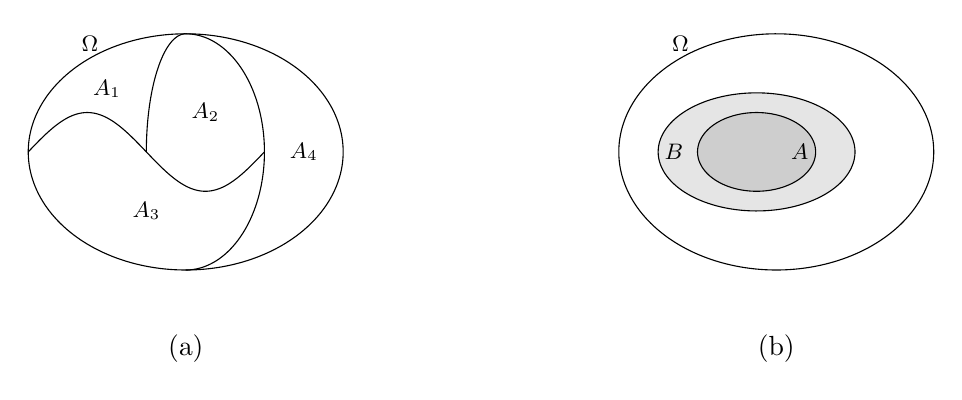
\begin{tikzpicture}%[scale=.9]
\shorthandoff{>}
%
% Particion
\begin{scope}
%
% Omega y A_i
\draw[domain=0:360,samples=200] plot ({2*cos(\x)+.5},{1.5*sin(\x)});
\draw[domain=-90:90,samples=200] plot ({cos(\x)+.5},{1.5*sin(\x)});
\draw[domain=90:180,samples=200] plot ({.5*cos(\x)+.5},{1.5*sin(\x)});
\draw[domain=0:3,samples=200] plot (\x-1.5,{.5*sin(120*\x)});
%
%
% Omega y A_i's
\draw(-.5,1.375) node[left,scale=.9]{\small $\Omega$};
\draw(-.5,.8) node[scale=.9]{\small $A_1$};
\draw(.75,.5) node[scale=.9]{\small $A_2$};
\draw(0,-.75) node[scale=.9]{\small $A_3$};
\draw(2,0) node[scale=.9]{\small $A_4$};
%
\draw (.5,-2.5) node{(a)};
\end{scope}
%
%
% Inclusion
\begin{scope}[xshift=7.5cm]
%
\fill[opacity=.1] plot[domain=0:360,samples=200] ({1.25*cos(\x)+.25},{.75*sin(\x)});
\fill[opacity=.1] plot[domain=0:360,samples=200] ({.75*cos(\x)+.25},{.5*sin(\x)});
%
% borders A, B y Omega
\draw[domain=0:360,samples=200] plot ({1.25*cos(\x)+.25},{.75*sin(\x)});
\draw[domain=0:360,samples=200] plot ({.75*cos(\x)+.25},{.5*sin(\x)});
\draw[domain=0:360,samples=200] plot ({2*cos(\x)+.5},{1.5*sin(\x)});
%
% A, B, Omega
\draw(.8,0) node[scale=.9]{\small $A$};
\draw (-.8,0) node[scale=.9]{\small $B$};
\draw(-.5,1.375) node[left,scale=.9]{\small $\Omega$};
%
\draw (.5,-2.5) node{(b)};
\end{scope}
%
\end{tikzpicture} \end{center}
%
\leyenda{Ilustraci\'on de: (a) conjunto completo de eventos posibles excluyentes
  entre s\'i;  (b) inclusi\'on  entre eventos, donde  $A$ est\'a en  gris oscuro
  mientras que $B$ est\'a en gris (claro y oscuro).}
\label{Fig:MP:CompletoSub}
\end{figure}

La probabilidad  \ $P(A \cap B)$  \ del evento $A  \cap B$ \  se llama tambi\'en
{\it probabilidad conjunta} de \ $A$ \ y \ $B$.  Se demuestra que
%
\begin{itemize}
\item $P(A  \cap B)$ est\'a acotada:  \ $0 \leq P(A  \cap B) \leq  \min\{ P(A) ,
  P(B)\}$ \ (viene de \ $A \cap B \subset A$ \ y \ $A \cap B \subset B$);
%
\item si $A$  y $B$ son mutuamente excluyentes,  entonces \ $P(A \cap B)  = 0$ \
  (viene de \ $A \cap B = \emptyset$);
%
\item  si  $\{ B_j  \}_{j=1}^m$  es un  conjunto  completo  de eventos  posibles
  excluyentes  entre s\'i,  entonces \  $\sum_{j=1}^m P(A  \cap B_j)  =  P(A)$ \
  (viene de $\{ A \cap B_j  \}_j$ mutuamente excluyentes y \ $\bigcup_j \left( A
    \cap B_j\right) = A \cap \left( \bigcup_j B_j \right) = A \cap \Omega = A$).
\end{itemize}

En el caso de eventos no necesariamente mutuamente excluyentes, se prueba que la
{\it ley de composici\'on} o {\it f\'ormula de inclusi\'on-exclusi\'on} es
%
\[
P(A \cup B) = P(A) + P(B) - P(A \cap B) \leq P(A) + P(B), 
\]
%
y que para $n$ eventos resulta
%
\[
P\left( \bigcup_{i=1}^n A_i \right) \leq \sum_{i=1}^n P\left( A_i \right).
\]
%
La  igualdad  vale  en  el  caso  especial  de  eventos  mutuamente  excluyentes
(recuperando el segundo axioma de Kolmogorov).

Se prueba tambi\'en  que si $\{ A_i \}_{i = 1}^{+\infty}$  es una secuencia {\it
  creciente} de  eventos, \ie $\forall \,  i \ge 1, \quad  A_i \subset A_{i+1}$,
entonces
%
\[
P\left( \bigcup_{i=1}^{+\infty} A_i \right) = \lim_{i \to +\infty} P(A_i).
\]
%
Por otro lado, si $\{ A_i \}_{i=1}^{+\infty}$ es una secuencia {\it decreciente}
de eventos, \ie $\forall \, i \ge 1, \quad A_{i+1} \subset A_i$, entonces
%
\[
P\left( \bigcap_{i=1}^{+\infty} A_i \right) = \lim_{i \to +\infty} P(A_i).
\]

Podemos preguntarnos cu\'al es la probabilidad  de un evento $A$, si sabemos que
se da  cierto evento~$B$.   Por ejemplo,  para un dado  de 6  caras equilibrado,
cu\'al  es la  probabilidad de  tener un  n\'umero par  sabiendo que  tenemos un
n\'umero menor o  igual a 3.  La  respuesta se encuentra en la  noci\'on de {\it
  probabilidad   condicional}~\cite{Hau01,   Jef48,   Jef73,  Bre88,   ManWol95,
  JacPro03, ShaVov06}:
%
\begin{definicion}[Probabilidad condicional]
\label{Def:MP:ProbaCondicional}
%
  La  {\it probabilidad  condicional} de  $A$  dado $B$,  denotado $P(A|B)$,  se
  define  como  la  raz\'on entre  la  probabilidad  del  evento conjunto  y  la
  probabilidad de que se d\'e $B$ (cuando \'este es un evento de probabilidad no
  nula):
  %
  \[
  P(A|B) = \frac{P(A \cap B)}{P(B)}.
  \]
\end{definicion}
%
En  el  ejemplo precedente,  la  probabilidad condicional  va  a  ser $P(A|B)  =
\frac{P(A \cup B)}{P(B)} = \frac{\frac16}{\frac12} = \frac13$.

Claramente  del  hecho  de  que  \  $P$  \ es  una  medida  de  probabilidad  se
tiene \[P(A|B) \ge 0.\] Luego, de \ $A \cap B \subseteq B$ \ resulta \ $P(A \cap
B) \le  P(B)$; es decir,  \[ P(A|B) \le  1. \] Adem\'as,  \ $P(\Omega \cap  B) =
P(B)$ \ dando  \[P(\Omega|B) = 1.\] Para  cualquier conjunto \ $\{ A_i  \}$ \ de
eventos  mutuamente  excluyentes,  los \  $\left(  A_i  \cap  B \right)$  \  son
tambi\'en  mutuamente excluyentes,  as\'i  que \  $\displaystyle P\left(  \left(
    \bigcup_i  A_i \right)  \bigcap B  \right)  = P\left(  \bigcup_i \left(  A_i
    \bigcap  B  \right)  \right) =  \sum_i  P\left(  A_i  \bigcap B  \right)$  \
dando \[P\left( \left.  \bigcup_i A_i  \right| B \right) = \sum_i P\left( \left.
    A_i \right|  B \right).\] Dicho  de otra manera,  $P(A|B)$ es una  medida de
probabilidad~\footnote{Se puede definir un  espacio de probabilidad $( \Omega_B,
  \A_B  , P_B)$  donde  $P_B(A)  \equiv P(A|B)$.  La  notaci\'on $P_B(A)$  suele
  utilizarse  en  la  literatura pero  no  la  usaremos  en  esta obra  para  no
  confundirla  con la  medida  de  probabilidad de  una  variable aleatoria  que
  definiremos   en   la   secci\'on   siguiente.}.   Diversas   situaciones   de
probabilidades condicionales son ilustradas en la Fig.~\ref{Fig:MP:Condicional}.

\begin{figure}[h!]
\begin{center} 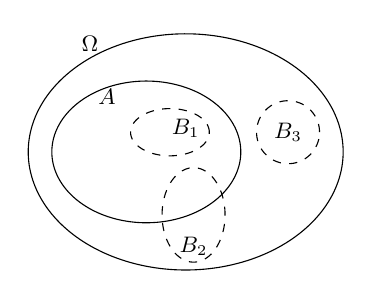
\begin{tikzpicture}%[scale=.9]
\shorthandoff{>}
%
\begin{scope}
%
% Omega, A, B_i
\draw[domain=0:360,samples=200] plot ({2*cos(\x)+.5},{1.5*sin(\x)});
\draw[domain=0:360,samples=200] plot ({1.2*cos(\x)},{.9*sin(\x)});
\draw[dashed,domain=0:360,samples=200] plot ({.5*cos(\x)+.3},{.3*sin(\x)+.25});
\draw[dashed,domain=0:360,samples=200] plot ({.4*cos(\x)+.6},{.6*sin(\x)-.8});
\draw[dashed,domain=0:360,samples=200] plot ({.4*cos(\x)+1.8},{.4*sin(\x)+.25});
%
%
% Omega y A_i's
\draw(-.5,1.375) node[left,scale=.9]{\small $\Omega$};
\draw(-.5,.7) node[scale=.9]{\small $A$};
\draw(.5,.3) node[scale=.9]{\small $B_1$};
\draw(.6,-1.2) node[scale=.9]{\small $B_2$};
\draw(1.8,.25) node[scale=.9]{\small $B_3$};
%
\end{scope}
%
\end{tikzpicture} \end{center}
%
\leyenda{Ilustraci\'on  de la probabilidad  condicional con  $A$ interior  de la
  curva  en l\'inea  llena y  unos $B_i$  interiores de  las curvas  en l\'ineas
  discontinuas. Se tiene \ $\omega \in B_1 \Rightarrow \omega \in A$ \ as\'i que
  \ $P(A|B_1) = 1$; por otro  lado, \ $\omega \in B_3 \Rightarrow \omega \not\in
  A$  \ as\'i  que  \ $P(A|B_3)  =  0$.  Entre  estas  situaciones extremas,  si
  $P(\bar{A}  \cap B_2)  \ne 0$  \ y  \ $P(A  \cap B_2)  \ne 0$  \ tenemos  $0 <
  P(A|B_2) < 1$ (se puede tomar el ejemplo de probabilidad de un evento iguale a
  su superficia  sobre la de  $\Omega$ para ver  estas propiedades en  este caso
  particular).}
\label{Fig:MP:Condicional}
\end{figure}

Algunas propiedades interesantes son las siguientes:
%
\begin{itemize}
\item $P(A \cap B | B) = P(A|B)$ \  \big(viene de $P(A \cap B \cap B) = P(A \cap
  B)$\big);
%
\item si $A$ \ y \ $B$ \ son mutuamente excluyentes, obviamente \ $P(A|B) = 0$;
%
\item si $B \subseteq C$, entonces \ $P(A  | B \cap C) = P(A|B)$ \ \big(viene de
  \ $P(A | B  \cap C) = \frac{P(A \cap B \cap C)}{P(B  \cap C)} = \frac{P(A \cap
    B)}{P(B)}$, \ pues\ $B \cap C = B$\big);
%
\item  condici\'on de  normalizaci\'on:  \ si  \  $\{ A_i  \}_{i=1}^n$  \ es  un
  conjunto completo  de resultados  posibles mutuamente excluyentes,  entonces \
  $\sum_{i=1}^n P(A_i|B) = 1$;
%
\item relaci\'on  entre probabilidades condicionales  inversas: \ $\displaystyle
  P(B|A)  = \frac{P(B)}{P(A)}  P(A|B)$, de  donde \  $P(A|B)$ \  y \  $P(B|A)$ \
  coinciden s\'olo cuando \ $A$ \ y \ $B$ \ tienen la misma probabilidad;
%
%\item {\it  f\'ormula de probabilidad  total}: \ si  $\{ B_j \}$ es  un conjunto
%  completo de eventos no nulos mutuamente excluyentes, entonces
%  %
%  \[
%  P(A) = \sum_j P(A|B_j) P(B_j) 
%  \]
%  %
%  \big(viene de \ $A = A \cap  \left( \bigcup_j B_j \right) = \bigcup_j \left( A
%    \cap B_j \right)$ \ donde los \ $A \cap B_j$ \ son mutuamente excluyentes, y
%  $P\left( A \cap B_j \right) = P(A|B_j) P(B_j)$\big) ;
%
%\item {\it  f\'ormula de Bayes}:  \ si  $\{ B_j \}$  es un conjunto  completo de
%  eventos no nulos mutuamente excluyentes, entonces
  %
%  \[
%  P(B_i|A) = \frac{P(A \cap B_i)}{P(A)} = \frac{P(A|B_i) P(B_i)}{\sum_j P(A|B_j)
%    P(B_j)};
%  \]
  %
\end{itemize}

\modif{Las dos propiedades importantes son  la f\'ormula de probabilidad total y
  la f\'ormula  de Bayes (ver~\cite{Bre88,  JacPro03, Bay63, Bar58}~\footnote{La
    obra  del  matem\'atico y  religioso  ingl\'es  Thomas  Bayes fue  de  hecho
    recopilada  y publicada  despu\'es de  su muerte  por Richard  Price.}). Les
  vamos a ver en forma de lemma:

\begin{teorema}[F\'ormula de probabilidad total]
\label{Teo:MP:ProbaTotalDiscreto}
%
  Sea \ $J \subseteq  \Nset$ \ y \ $\{ B_j \}_{j \in  J}$ \ un conjunto completo
  de eventos  no nulos  mutuamente excluyentes, \ie  tal que  \ $B_i \cap  B_j =
  \emptyset$  \ si  \ $i  \ne j$  \ y  \ $\displaystyle  \bigcup_{j\in J}  B_j =
  \Omega$. Entonces
  %
  \[
  P(A) = \sum_{j \in J} P(A|B_j) P(B_j) 
  \]
\end{teorema}
%
\begin{proof}
  Escribimos \  $A = A  \cap \left( \bigcup_j  B_j \right) = \bigcup_j  \left( A
    \cap  B_j \right)$.  Los \  $A  \cap B_j$  \ son  mutuamente excluyentes,  y
  $P\left( A \cap B_j \right) = P(A|B_j) P(B_j)$ \ lo que cierra la prueba.
\end{proof}


\begin{lema}[F\'ormula de Bayes]\label{Lem:MP:BayesDiscreto}
%
  Sea \ $J \subseteq  \Nset$ \ y \ $\{ B_j \}_{j \in  J}$ \ un conjunto completo
  de eventos  no nulos  mutuamente excluyentes. Entonces
  %
  \[
  P(B_i|A) = \frac{P(A \cap B_i)}{P(A)} = \frac{P(A|B_i) P(B_i)}{\sum_{j \in J} P(A|B_j)
    P(B_j)};
  \]
\end{lema}
%
\begin{proof}
  Esta f\'ormula resuelta de la definici\'on de la probabilidad condicional y de
  la f\'ormula de probabilidad total.
\end{proof}
}

Veamos ahora la noci\'on de independencia  entre dos eventos. Por ejemplo, si se
tiran dos dados  sobre sendas mesas, no hay ninguna raz\'on  para que la muestra
de  uno  ``influya''  la  del  otro.  Dicho de  otra  manera,  dos  eventos  son
independientes  si el  conocimiento de  uno no  lleva  ninguna ``informaci\'on''
sobre el otro~\cite{Bre88, ManWol95, Hau01, JacPro03, Bor09}:
%
\begin{definicion}[Independencia estad\'istica]
\label{Def:MP:IndependenciaEtadistica}
%
  Dos eventos \ $A$ \ y \ $B$ \ se dicen {\it estad\'isticamente independientes}
  si la  probabilidad condicional  de $A$  dado $B$ es  igual a  la probabilidad
  incondicional de $A$:
  %
  \[
   P(A|B) = P(A).
   \]
  %
   Es equivalente al hecho de que la probabilidad conjunta se factoriza: 
  %
  \[
   P(A \cap B) = P(A) P(B).
   \]
\end{definicion}
%
Por  inducci\'on, la  condici\'on necesaria  y suficiente  para que  $n$ eventos
$A_1,\ldots,A_n$  sean mutuamente  estad\'isticamente independientes  es  que la
probabilidad conjunta se factorice como
%
\[
P\left( \bigcap_{i=1}^n A_i \right) = \prod_{i=1}^n P(A_i).
\]
%
Se  deduce que  los  eventos mutuamente  excluyentes  no son  estad\'isticamente
independientes.

Es  importante  notar  que  la  independencia  mutua  no  es  equivalente  a  la
independencia por pares de eventos, como lo ilustra el ejemplo siguiente.
%
\begin{ejemplo}[Independencia   mutua   vs    por   pares]
\label{Ej:MP:IndependenciaMutuaVsPares}
%
  Tiramos 2 dados independientemente y consideramos  los eventos: \ $A_i, i = 1,
  2$ \ ``el  dado $i$ es par'' y  $A_3$ ``la suma de ambos dados  es impar''. Es
  claro que \ $A_1$  \ y \ $A_2$ \ son independientes y adem\'as  para $i = 1$ o
  2, \ $P(A_i \cap A_3) = \frac14 = P(A_i) P(A_3)$, \ mientras que \ $P(A_1 \cap
  A_2 \cap A_3) = 0 \ne \frac18$: los eventos son independientes por pares, pero
  no son mutuamente independientes~\cite{HogMck13}.
\end{ejemplo}

\begin{definicion}[Independencia condicional]
\label{Def:MP:IndependenciaCondicional}
%
  Dos eventos \ $A$ \ y  \ $B$ \ se dicen {\it estad\'isticamente independientes
    condicionalmente} a un tercer evento  $C$, si la probabilidad conjunta de \
  $A$  \ y  \ $B$  \ condicionalmente  a  \ $C$  \ es  igual al  producto de  la
  probabilidad de  $A$ condicionalmente a $C$  por la de  $B$ condicionalmente a
  $C$:
  %
  \[
   P(A \cap B | C) = P(A | C) P(B |C).
   \]
   %
   Si $P(B|C) \ne 0$, es equivalente a $P(A|B \cap C) = P(A|C)$.
\end{definicion}
%
Es importante  notar  que dos  eventos pueden ser independientes,  pero no serlo
condicionalmente a un tercero, como lo ilustra el ejemplo siguiente.
%
\begin{ejemplo}[Independencia  incondicional pero  no condicional]
\label{Ej:MP:IndependenciaIncondicional}
%
  Teniendo dos monedas bien equilibradas y tir\'andolas de manera independiente,
  consideramos  los eventos  \ $A$  ``la  primera faz  es una  cruz'', $B$  ``la
  segunda faz  es una  cara'', $C$ ``las  faces son id\'enticas''.  Claramente \
  $P(A \cap B) = \frac14 = P(A) P(B)$, \ mientras que \ $P(A \cap B | C) = 0 \ne
  P(A|C) P(B|C) = \frac1{16}$.
\end{ejemplo}

Al rev\'es, dos eventos pueden ser condicionalmente independientes a un tercero,
pero  ser  dependientes.
%
\begin{ejemplo}[Independencia  condicional  pero  no  incondicional]
\label{Ej:MP:IndependenciaCondicional}
%
  Sea Alice tirando una moneda bien  equilibrada y denotamos $A$ el evento ``era
  una cruz''.   Claramente $P(A) =  \frac12$.  Suponemos que Alice  transmite el
  resultado a  Bob a trav\'es de  un intermediario Charlie  con una probabilidad
  $\varepsilon$ de  mentir a Charlie,  y llamamos $C$  el evento ``Alice  dijo a
  Charlie   que  era  una   cruz''.   Tenemos   que  $P(C)   =  P(C|A)   P(A)  +
  P(C|\widebar{A})  P(\widebar{A})  =   (1-\varepsilon)  \frac12  +  \varepsilon
  \frac12 =  \frac12$.  Suponemos ahora  que Charlie transmite  a Bob lo  que le
  dijo Alice, con una  probabilidad $\vartheta$ de mentir (independientemente de
  Alice) y llamamos $B$ el evento ``Charlie dijo a Bob que era una cruz''. Es de
  nuevo sencillo ver  que $P(B) = \frac12$.  Ahora, $P(A \cap  B |C) = \frac{P(A
    \cap B \cap C)}{P(C)} = 2 \, P(A \cap B \cap C)$. El evento \ $A \cap B \cap
  C$ \ es  era una cruz y Alice  no mint\'o y Charlie tampoco, es  decir, por la
  independencia:    $P(A   \cap    B   |C)    =   (1-\varepsilon)(1-\vartheta)$.
  Inmediatamente $P(B|C)  = 1-\vartheta$ \  y \  $P(A|C) = 2  \, P(A \cap  C)$ \
  siendo  \ $A  \cap  C$ \  el  evento ``era  una cruz  y  Alice no  minti\'o'',
  i.e. $P(A|C)  = 1-\varepsilon$. En  conclusi\'on, \ $P(A  \cap B |C)  = P(A|C)
  P(B|C)$: $A$  y $B$  son independientes condicionalmente  a $C$.   Ahora, $P(A
  \cap  B) =  P(A \cap  B  \cap C)  + P(A  \cap  B \cap  \widebar{C}) =  \frac12
  (1-\varepsilon)(1-\vartheta)  + \frac12  \varepsilon \vartheta  \ne  \frac14 =
  P(A) P(B)$ en  general: $A$ y $B$ no resultan  independientes. Este ejemplo es
  una instancia de lo que se llama un proceso de Markov, que vamos a ver un poco
  m\'as en el c\'apitulo~\ref{Cap:SZ:Informacion}.
\end{ejemplo}
